
%%%%%%%%%%%%%%%%%%%%%%% file typeinst.tex %%%%%%%%%%%%%%%%%%%%%%%%%
%
% This is the LaTeX source for the instructions to authors using
% the LaTeX document class 'llncs.cls' for contributions to
% the Lecture Notes in Computer Sciences series.
% http://www.springer.com/lncs       Springer Heidelberg 2006/05/04
%
% It may be used as a template for your own input - copy it
% to a new file with a new name and use it as the basis
% for your article.
%
% NB: the document class 'llncs' has its own and detailed documentation, see
% ftp://ftp.springer.de/data/pubftp/pub/tex/latex/llncs/latex2e/llncsdoc.pdf
%
%%%%%%%%%%%%%%%%%%%%%%%%%%%%%%%%%%%%%%%%%%%%%%%%%%%%%%%%%%%%%%%%%%%


\documentclass[runningheads,a4paper]{llncs}

\usepackage{amssymb}
\setcounter{tocdepth}{3}
\usepackage{graphicx}

\usepackage[portuguese]{babel}
\usepackage[utf8]{inputenc}

\usepackage{url}
\urldef{\mailsa}\path|{alfred.hofmann, ursula.barth, ingrid.haas, frank.holzwarth,|
\urldef{\mailsb}\path|anna.kramer, leonie.kunz, christine.reiss, nicole.sator,|
\urldef{\mailsc}\path|erika.siebert-cole, peter.strasser, lncs}@springer.com|    
\newcommand{\keywords}[1]{\par\addvspace\baselineskip
\noindent\keywordname\enspace\ignorespaces#1}

\begin{document}

\mainmatter  % start of an individual contribution

% first the title is needed
\title{Lecture Notes in Computer Science:\\Authors' Instructions
for the Preparation\\of Camera-Ready
Contributions\\to LNCS/LNAI/LNBI Proceedings}

% a short form should be given in case it is too long for the running head
\titlerunning{Lecture Notes in Computer Science: Authors' Instructions}

% the name(s) of the author(s) follow(s) next
%
% NB: Chinese authors should write their first names(s) in front of
% their surnames. This ensures that the names appear correctly in
% the running heads and the author index.
%
\author{Alfred Hofmann%
\thanks{Please note that the LNCS Editorial assumes that all authors have used
the western naming convention, with given names preceding surnames. This determines
the structure of the names in the running heads and the author index.}%
\and Ursula Barth\and Ingrid Haas\and Frank Holzwarth\and\\
Anna Kramer\and Leonie Kunz\and Christine Rei\ss\and\\
Nicole Sator\and Erika Siebert-Cole\and Peter Stra\ss er}
%
\authorrunning{Lecture Notes in Computer Science: Authors' Instructions}
% (feature abused for this document to repeat the title also on left hand pages)

% the affiliations are given next; don't give your e-mail address
% unless you accept that it will be published
\institute{Springer-Verlag, Computer Science Editorial,\\
Tiergartenstr. 17, 69121 Heidelberg, Germany\\
\mailsa\\
\mailsb\\
\mailsc\\
\url{http://www.springer.com/lncs}}

%
% NB: a more complex sample for affiliations and the mapping to the
% corresponding authors can be found in the file "llncs.dem"
% (search for the string "\mainmatter" where a contribution starts).
% "llncs.dem" accompanies the document class "llncs.cls".
%

\toctitle{Lecture Notes in Computer Science}
\tocauthor{Authors' Instructions}
\maketitle


\begin{abstract}
The abstract should summarize the contents of the paper and should
contain at least 70 and at most 150 words. It should be written using the
\emph{abstract} environment.
\keywords{We would like to encourage you to list your keywords within
the abstract section}
\end{abstract}


\section{Introdução}

\section{Diferenças da especificação}

O protocolo implementado segue o proposto no enunciado com duas diferenças.
Na lista de argumentos de uma PDU tinha o tamanho do parâmetro. Estava previsto que este tamanho apenas tivesse 1 bytes, mas isto não era suficiente por exemplo no caso do bloco de musica. Portanto modificou-se para 2 bytes.
Adicionou-se também um tipo de PDU de controlo para os servidores fecharem os sockets em segurança. 

\section{Implementação}

\subsection{Protocolo}


\begin{figure}
\centering
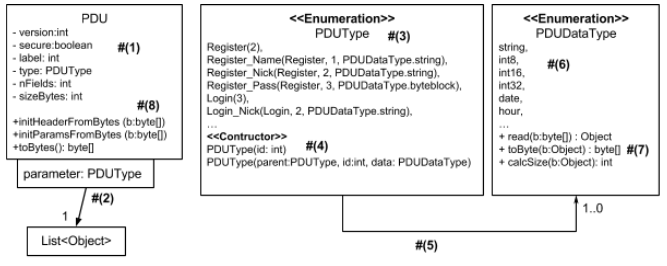
\includegraphics[height=6.2cm]{UDP.png}
\caption{Diagrama UMP da interpretação de PDU}
\label{fig:diagram-pdu}
\end{figure}

Para a abstração dos Bits, foi criada a classe PDU, que é capaz de criar as PDU’s e depois transformas em Bytes e também inicializar-se através de array de Bytes.
Internamente existem os parâmetros do cabeçalho da PDU [\#(1)] (versão, segurança, label, tipo da PDU, número de campos e tamanho tamanho total dos campos em Bytes), toda esta informação pode ser consultada com os seus respetivos métodos.
Para guardar os campos da PDU, utiliza-se um Map [\#(2)] onde a chave é o tipo do campo e o valor é uma lista de valores. Uma lista porque a mesma PDU pode ter varias campos com o mesmo tipo como é o exemplo de uma questão que têm varias respostas.

A Enumeração PDUType [\#(3)] é uma enumeração hierárquica, isto é: existem os valores de origem que representam o tipo da PDU como por exemplo: Register, Login, Replay. Depois existem os valores que representam os campos, como por exemplo: Register\_Name ou Register\_Nick.
A Diferença entre estes dois está no construtor utilizada [\#(4)]. No caso do construtor de um campo podemos reparar que recebe um tipo de dados (PDUDataType).

A enumeração PDUDataType [\#(6)] tem todos os tipos de dados que o PDU suposta, e aqui ficam implementadas as funções de leitura e conversão para arrays de bytes.
Desta forma é fácil a adição de novos tipos de dados.

O diagrama \ref{fig:diagram-pdu} UML explica o funcionamento da interpretação do campos do PDU (função initParamsFromBytes).

\begin{figure}
\centering
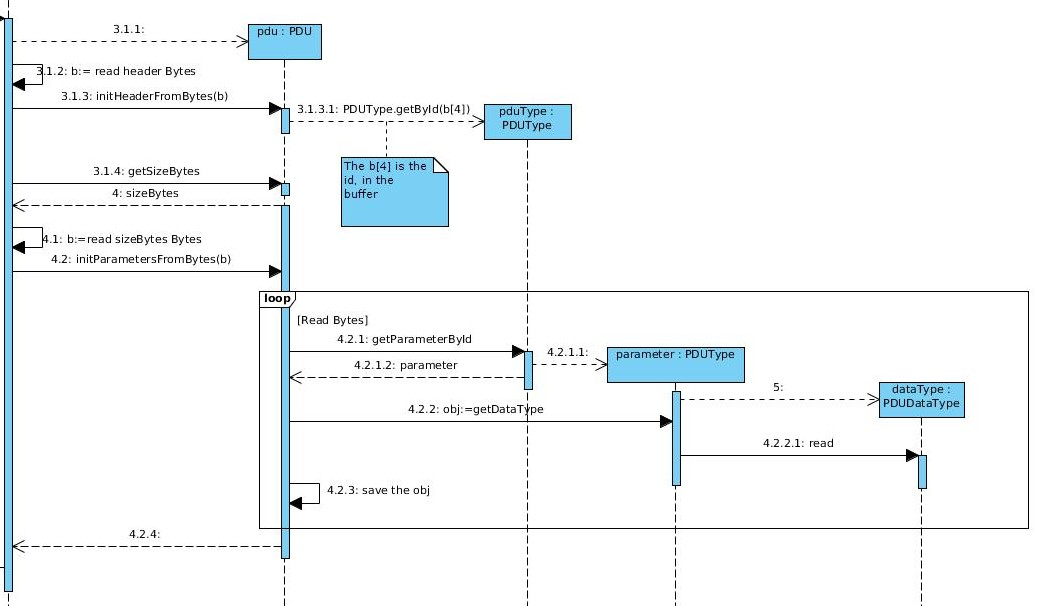
\includegraphics[height=6.2cm]{PDU_interpretation.jpg}
\caption{Diagrama UMP da interpretação de PDU}
\label{fig:diagram-pdu}
\end{figure}

\subsection{Cliente}

\subsection{Servidor}

O Servidor é responsável guardar a informação sobre do sistema tais como os desafios e utilizadores existentes. Por outro lado o servidor também é responsável por partilhar o seu conhecimento com os outros servidores.
No arranque o servidor cria 2 threads, um deles para atender clientes, e outro para atender outros  servidores 

A arquitetura geral de um servidor posso ser vista no diagrama \ref{fig:diagram-arq-geral}.

\begin{figure}
\centering
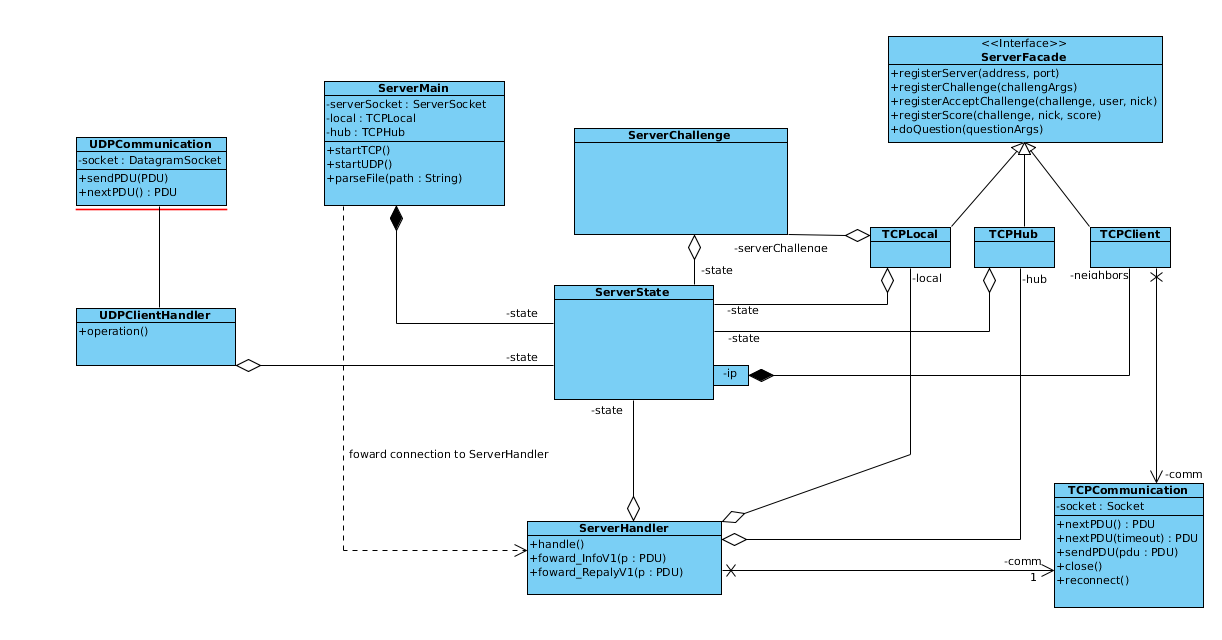
\includegraphics[height=6.2cm]{arq-geral.png}
\caption{Diagrama UML da arquitetura do servidor}
\label{fig:diagram-arq-geral}
\end{figure}


\subsubsection{Dados Guardados}

Toda a informação é guardada na classe ServerState, aqui são guardados:
\begin{itemize}
  \item Utilizadores identificados por o seu nick
  \item Sessões, guardam os utilizadores identificados por o seu ip actual
  \item Utilizadores globais, para guarda o ranking global do sistema.
  \item Desafios identificados por o seu nome
  \item Questões para criar novos desafios, identificados por o seu ip
  \item Servidores vizinhos poder comunicar.
\end{itemize}

No caso dos desafios cada desafio tem: o ranking atual dos utilizadores inscritos nesse desafio, os utilizadores e servidores subscritos e as questões selecionadas.

\subsubsection{Atender Clientes}

Um pedido vindo de um cliente é reencaminhado para a class UDPClientHandler, aqui mediante o tipo de desafio, é realizada as regras de negocio correspondente e enviada uma resposta para o cliente.

Existem alguns pedidos do cliente que podem gerar que o servidor que esteja a antender tenha que informar os restantes servidores como por exemplo: makeChallenge, que inicia um desafio e irá ser explicado de seguida. 
Iniciar desafio

Quando um makeChallenge e gerado, o sistema cria uma nova thread que terá um temporalizador para correr às horas pretendidas.

Quando esta thread inicia o seu processo confirma que existem pessoas suficientes no desafio, caso não existam cancela o desafio. Caso esteja tudo bem continua e envia a primeira pergunta.

As perguntas ao longo do desafio são enviadas para todos os clientes subscritos e para todos os servidores subscritos, depois cada um destes servidores reencainhará para os clientes finais.

\subsubsection{Atender Servidores}

O processo de atender servidores é semelhante ao de atender clientes.  Os pedidos são interpretados na class ServerHandler, esta class mediante os parametros existentes irá executar a logica de negocio necessária.
O negocio está implementado em 3 classes distintas: TCPLocal, TCPHub e TCPClient. cada uma destas implementam a interface ServerToServerFacade que especifica todos os métodos existentes no negocio da aplicação.
Cada uma das implementações implementa o negocio de forma diferente:
\begin{itemize}
\item TCPLocal aplica as regras de negocio na propria maquina.
\item TCPClient aplica as regras de negocio a um servidor.
\item TCPHub aplica as regras de negocio a todos os servidores chamando o TCPClient de cada servidor.
\end{itemize}

O socket que permite a comunicação entre servidores é terminado com um timeout parameterizavel.

\begin{figure}
\centering
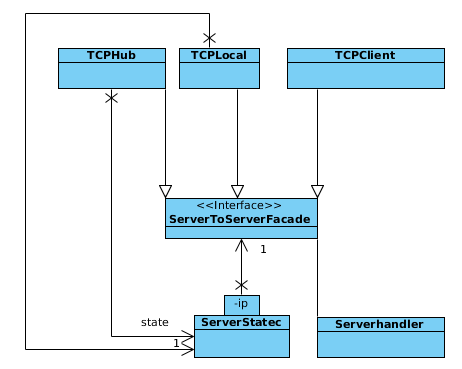
\includegraphics[height=6.2cm]{facades.png}
\caption{Diagrama UML da arquitetura do servidor}
\label{fig:diagram-facades}
\end{figure}


\subsubsection{Informar Servidores}
Como se envia PDU’s info para outro servidor.


\section{Testes Realizados}

\end{document}
